\documentclass[aspectratio=169]{audition-beamer}

\usepackage[francais]{babel}
\input{preamble}
% Adapted from https://tex.stackexchange.com/a/396754/28146

% \setbeameroption{show notes on second screen}
\draft
% \webcast
% \setbeamercolor{alerted text}{fg=supelecRed!20!red!80}
% \usetikzlibrary{overlay-beamer-styles}
% \includeonlyframes{current,current1,current2,current3,current4,current5,current6,current7}

\bibliography{bibliography.bib}

\title[Discuter] % (optional, use only with long paper titles)
{Discuter:}

\subtitle
{Ontologies + NLP + Minecraft = ?}

\author[Rafael Accácio Nogueira] % (optional, use only with lots of authors)
{Rafael Accácio NOGUEIRA\\
  \texttt{rafael.accacio.nogueira@gmail.com}}

% \institute[IETR --- CentraleSupélec] % (optional, but mostly needed)
% {
% }


\day29 \month08 \year2024
\makeatletter
\date{\@date\ @ Toulouse}
\makeatother
% {\textbf{Audition MCF 4101 0067 \\École Centrale de Lyon / Laboratoire Ampère}
%   \\
%   30 mai 2023 @ Écully\\
%   % \begin{minipage}{.3\textwidth}
%   %   \centering
%   %   %   \includegraphics[width=2cm]{logos/IETR_2022.png}
%   % \end{minipage}
%   % \hfill
%   \begin{minipage}{\textwidth}
%     \centering
%     \vspace{10pt}
%     \includegraphics[width=1.5cm]{qrPresentation.png}
%     % qrencode https://gitlab.com/Accacio/audition_mcf_2023/-/raw/main/presentation.pdf -o ~/git/SysTol21/img/qrPresentation.png
%     % \href{https://bit.ly/3g3S6X4}{https://bit.ly/3g3S6X4}
%   \end{minipage}
%   % \begin{minipage}{.3\textwidth}
%   %   \centering
%   %   \vspace{10pt}
%   %   %   \includegraphics[width=2cm]{logos/supelec.jpeg}
%   % \end{minipage}
% }
% % - Either use conference name or its abbreviation.
% % - Not really informative to the audience, more for people (including
% % yourself) who are reading the slides online

% \subject{}

% % \logo{\includegraphics[width=1.5cm]{logos/supelec.jpeg}}

% % Delete this, if you do not want the table of contents to pop up at
% % the beginning of each subsection:
\AtBeginSection[]
{
  \begin{frame}<beamer>{Sommaire}
    \tableofcontents[sectionstyle=show/hide,subsectionstyle=show/show/hide]
  \end{frame}
}

\begin{document}

\begin{frame}[plain]
  \titlepage%
\end{frame}

% \begin{frame}[plain]
%   \titlepage%
%   \note{45 minutes !!!!\\}
%   \script{Good afternoon, thank you all for being here.}
%   \script{I'm Rafael Accácio and I'm going to present my work on the security of distributed model predictive control under false data injection.}
% \end{frame}


\begin{frame}{DISCUTER}
{\color{auditionPrimary} D}ialogue Interactif Structuré, Consolidé et Unifié\\ pour la réalisation de Tâches En Robotique\pause
\\~\\
Étudier la collaboration entre agents pour des tâches complexes.
\\~\\
\pause Associer \pause
\begin{itemize}
  \item Traitement automatique des langues (NLP)\pause
  \item Théorie de l'esprit
\end{itemize}
\end{frame}

\begin{frame}{Collaborative Dialogue}
{\small \cite{Narayan-ChenEtAl2019}}
2 agents: 1 architect et 1 constructeur
\end{frame}


\begin{frame}{Sommaire}
  % \tableofcontents
  \tableofcontents[subsectionstyle=hide/hide/hide]

\end{frame}


\begin{frame}{État}
Ismail

\begin{itemize}
  \item Enregistrement de l'état en fichiers \texttt{.json}
  \item Replay de l'état en créant
\end{itemize}
\end{frame}


\section{Tâches}

% \begin{frame}{Parcours Académique}
%   \only<2>{
%     \begin{minipage}[c]{.7\linewidth}
%       \begin{itemize}
%         \item[] Techn. Électron. Analog. et Numérique --- CEFET-RJ\\ (2010--2013)
%       \end{itemize}
%     \end{minipage}
%     \hfill
%     \begin{minipage}[c]{.2\linewidth}
%       \centering
%       \includegraphics[width=3cm]{logos/cefet.jpg}%
%     \end{minipage}
%   }
%   \only<3>{
%     \vspace{-1cm}
%     \begin{minipage}[c]{.7\linewidth}
%       \begin{itemize}
%         \item[] B.Sc Ingérierie de Contrôle et Automatismes --- UFRJ\\ (2013--2019)
%         \item[] Ing. Ingérierie de Systèmes Automatisés --- Supélec\\ (2016--2018)
%         \item[] Master Recherche SISEA --- UR1/CS\\ (2017--2018)
%       \end{itemize}
%     \end{minipage}
%     \hfill
%     \begin{minipage}[c]{.2\linewidth}
%       \centering
%       \includegraphics[width=3cm]{logos/poli-ufrj.png}%

%       \includegraphics[width=3cm]{logos/supelec.jpeg}%

%       \includegraphics[width=3cm]{logos/rennes1.png}%
%     \end{minipage}
%   }

%   \only<4>{
%     \vspace{-1cm}
%     \begin{minipage}[c]{.7\linewidth}
%       \begin{itemize}
%         \item[] Ph.D. Automatique, Robot., Produt. --- UR1/CS\\ (2019--2022)
%       \end{itemize}
%     \end{minipage}
%     \hfill
%     \begin{minipage}[c]{.2\linewidth}
%       \centering
%       \includegraphics[width=3cm]{logos/supelec.jpeg}%

%       \includegraphics[width=3cm]{logos/rennes1.png}%
%     \end{minipage}
%   }

%   \begin{tikzpicture}[overlay, remember picture]
%     \node[anchor=south] (image) at (current page.south) {\includegraphics<1>[width=\textwidth]{timeline_1.pdf}};
%     \node[anchor=south] (image) at (current page.south) {\includegraphics<2>[width=\textwidth]{timeline_2.pdf}};
%     \node[anchor=south] (image) at (current page.south) {\includegraphics<3>[width=\textwidth]{timeline_5.pdf}};
%     \node[anchor=south] (image) at (current page.south) {\includegraphics<4>[width=\textwidth]{timeline_6.pdf}};
%   \end{tikzpicture}
% \end{frame}

% \section{Recherche}

% \definecolor{neocampus_yellow}{RGB}{255, 159, 0}
% \definecolor{neocampus_bright_yellow}{RGB}{255, 207, 128}
% \newcommand{\autOCampus}{aut{\color{neocampus_yellow}O\!\!C}ampus}
% \newcommand{\neOCampus}{ne{\color{neocampus_yellow}O\!\!C}ampus}

% \begin{frame}{Expérience en Recherche}
%   \begin{overlayarea}{\textwidth}{5cm}
%   \only<2>{
%     \begin{minipage}[c]{.75\linewidth}
%       \begin{itemize}
%         \item[] Init. à la Rech. --- LAPIS (Coppe/UFRJ) (2015--2016)
%         \item[] \textit{Contrôle d'orthèses pour patients avec atrophie musc.}
%         \item[] Supervisionné par C. J. Tierra Criollo
%       \end{itemize}

%       % \centering
%       \begin{minipage}[c]{.2454\textwidth}
%         \centering
%         \includegraphics[width=.8\textwidth]{bras_prototype.jpg}%
%       \end{minipage}
%     \hfill
%     \tikz\draw[{latex}-{latex}] (0,0) - +(.0818181\textwidth,0) node [midway,above,align=center] {};%
%     \hfill
%       \begin{minipage}[c]{.2454\textwidth}
%         \centering
%         \includegraphics[width=.7\textwidth]{arduino-UNO.png}%
%       \end{minipage}
%     \hfill
%     \tikz\draw[{latex}-{latex}] (0,0) - +(.0818181\textwidth,0) node [midway,above,align=center] {};%
%     \hfill
%       \begin{minipage}[c]{.2454\textwidth}
%         \centering
%         \includegraphics[width=.7\textwidth]{Matlab_Logo}%
%       \end{minipage}
%     \end{minipage}
%     \hfill
%     \begin{minipage}[c]{.2\linewidth}
%       \centering
%       \tikz\node[fill=auditionPrimary!90] (a) {\includegraphics[width=2.3cm]{logos/logo-coppe-50.png}
%       };%

%         \includegraphics[width=2.3cm]{LogoPEB.png}
%     \end{minipage}
%   }

%   \only<3>{
%     \begin{minipage}[c]{.7\linewidth}
%       \begin{itemize}
%         \item[] Stage 2A --- AUTO IETR (2017--2017)
%         \item[] \textit{Contrôle d'un réseau de distribution d'électricité}
%         \item[] Supervisionné par Hervé Guéguen
%       \end{itemize}


%     \begin{minipage}[c]{.2454\textwidth}
%       \centering
%       \includegraphics[width=1\textwidth]{reseau_dist.pdf}
%     \end{minipage}%
%     \hfill
%     \tikz\draw[-{latex}] (0,0) - +(.0818181\textwidth,0) node [midway,above,align=center] {};%
%     \hfill
%     \begin{minipage}[c]{.2454\textwidth}
%       \centering
%       $Q(U)$\\

%       \includegraphics[width=1.0\textwidth]{regulateur.pdf}
%     \end{minipage}
%     \hfill
%     \tikz\draw[-{latex}] (0,0) - +(.0818181\textwidth,0) node [midway,above,align=center] {};%
%     \hfill
%     \begin{minipage}[c]{.2454\textwidth}
%       \centering
%       \includegraphics[width=1\textwidth]{controle_tension_distribution_network.pdf}
%     \end{minipage}

%     \end{minipage}
%     \hfill
%     \begin{minipage}[c]{.2\linewidth}
%       \centering
%       \includegraphics[width=3cm]{logos/IETR_2022.png}%
%     \end{minipage}
%   }
%   \only<4>{
%     % \vspace{-1cm}
%     \begin{minipage}[c]{.7\linewidth}
%       \begin{itemize}
%         \item[] Stage 3A --- Renault (2018--2018)
%         \item[] \textit{Superviseur pour véhicule autonome}
%         \item[] Supervisionné par F. Shokry
%       \end{itemize}

% \vspace{.5cm}
%       \centering
%     \begin{minipage}[c]{.2454\textwidth}
%       \centering
%       \includegraphics[width=1.0\textwidth]{stateflow.png}
%     \end{minipage}%
%     \hfill
%     \tikz\draw[-{latex}] (0,0) - +(.0818181\textwidth,0) node [midway,above,align=center] {};%
%     \hfill
%     \begin{minipage}[c]{.2454\textwidth}
%       \centering
%       \includegraphics[width=1\textwidth]{microAutoBox.jpeg}
%     \end{minipage}
%     \hfill
%     \tikz\draw[-{latex}] (0,0) - +(.0818181\textwidth,0) node [midway,above,align=center] {};%
%     \hfill
%     \begin{minipage}[c]{.2454\textwidth}
%       \centering
%       \includegraphics[width=1\textwidth]{zoe.png}
%     \end{minipage}
%     \end{minipage}
%     \hfill
%     \begin{minipage}[c]{.2\linewidth}
%       \centering
%       \includegraphics[width=2cm]{logos/renault.jpg}%

%     \end{minipage}
%   }

%   \only<5>{
%     \begin{minipage}[c]{.7\linewidth}
%       \begin{itemize}
%         \item[] Recherche B.Sc --- LCA (Coppe/UFRJ) (2019--2019)
%         \item[] \textit{Identif. des syst. industriels pour la détection de failles}
%         \item[] Supervisionné par M. V. de Brito Moreira
%       \end{itemize}
%       \centering
%       \begin{minipage}[c]{.4\textwidth}
%         \includegraphics[width=.3\textwidth]{maquete/mag.jpg}
%         \includegraphics[width=.3\textwidth]{maquete/esteira.jpg}
%         \includegraphics[width=.3\textwidth]{maquete/sensores.jpg}

%         \includegraphics[width=.3\textwidth]{maquete/braco.jpg}
%         \includegraphics[width=.3\textwidth]{maquete/prensa.jpg}
%         \includegraphics[width=.3\textwidth]{maquete/elevador.jpg}
%       \end{minipage}
%       \resizebox{.1\textwidth}{!}{\tikz\draw[->] (0,0) - +(2,0) node [midway,above,align=center] {I/O\\ +\\ DAOCT};}
%       \begin{minipage}[c]{.4\textwidth}
%         \includegraphics[width=\textwidth]{maquete/example.pdf}
%       \end{minipage}
%     \end{minipage}
%     \hfill
%     \begin{minipage}[c]{.2\linewidth}
%       \centering
%       \tikz\node[fill=auditionPrimary!90] (a) {\includegraphics[width=2.3cm]{logos/logo-coppe-50.png}};%


%       \includegraphics[width=2.3cm]{LogoLCA.png}
%     \end{minipage}
%   }

%   \only<6>{
%     \begin{minipage}[c]{.7\linewidth}
%       \begin{itemize}
%         \item[] Ph.D  --- AUTO IETR (2019--2022)
%         \item[] \textit{Sécurité de la dMPC contre injection de données}
%         \item[] Supervisionné par H. Guéguen et R. Bourdais
%       \end{itemize}

%       \centering
%       \includegraphics[width=5cm]{Non-coop_Agent_1.png}%
%     \end{minipage}
%     \hfill
%     \begin{minipage}[c]{.2\linewidth}
%       \centering
%       \includegraphics[width=3cm]{logos/IETR_2022.png}%
%     \end{minipage}
%   }

%   \only<7>{
%     \begin{minipage}[c]{.7\linewidth}
%       \begin{itemize}
%         \item[] Post-doc --- LAAS/CNRS (2023--2024)
%         \item[] \textit{Localisation garantie de véhicules autonomes}
%         \item[] Supervisionné par Soheib Fergani (DISCO)
%       \end{itemize}

%       \centering
%       % \vspace{1cm}
%       \resizebox{!}{3cm}{
%         \begin{tikzpicture}
%           % \draw [help lines] (-1,-1) grid [step=.1cm] (1,1);
%           \node[] (car_purple_position) {};

%           % constrained zonotope
%           \draw[neocampus_yellow,fill=neocampus_yellow] (-0.65,-0.1) -- ++(90:0.2) -- ++(45:0.42) --++(0:0.4) -- ++(-30:0.53) -- ++(-90:0.32) -- ++(210:0.28) --++(180:0.45) --++(160:0.49) -- cycle;

%           \path[draw,use Hobby shortcut,closed=true,violet!50!white]
%           % \path[draw,use Hobby shortcut,closed=true,violet!50!white,fill=violet!50!white,opacity=0.5]
%           ($(car_purple_position)+(.5,0)$) .. ++(-.3,.3) .. ++(-.1,.05) .. ++(-0.6,-0.1) ..++(-0.1,-0.4) ..++(0.2,-0.1);
%           \node[] (car_purple) at (car_purple_position) {\includegraphics[height=1cm,angle=90]{car_purple}};

%         \end{tikzpicture}
%       }
%     \end{minipage}
%     \hfill
%     \begin{minipage}[c]{.2\linewidth}
%       \centering
%       \includegraphics[width=3cm]{logos/laas.png}%

%     \end{minipage}
%   }

%   \only<8>{
%     \begin{minipage}[c]{.7\linewidth}
%       \begin{itemize}
%         \item[] Ingénieur de Recherche --- LAAS/CNRS (2024--2024)
%         \item[] \textit{Ontologies + langage naturel}
%         \item[] Supervisionné par Aurélie Clodic (RIS)
%       \end{itemize}


%       \centering
%       % \vspace{1cm}
%       \resizebox{!}{1.7cm}{
%       \begin{minipage}[c]{.2\linewidth}
%         \centering
%         \includegraphics[width=.8\textwidth]{Ros_logo.png}%

%         \includegraphics[width=.5\textwidth]{overworld.png}%

%         \small LLaMIPa
%       \end{minipage}
%     % \hfill
%     \tikz\draw[{latex}-{latex}] (0,0) - +(.05\textwidth,0) node [midway,above,align=center] {};%
%     % \hfill
%       \begin{minipage}[c]{.2\linewidth}
%         \centering
%         \includegraphics[width=.8\textwidth]{Steve_Alex.jpg}%
%       \end{minipage}
%     % \hfill
%     \tikz\draw[-{latex}] (0,0) - +(.05\textwidth,0) node [midway,above,align=center] {};%
%     % \hfill
%       \begin{minipage}[c]{.2\linewidth}
%         \centering
%         \includegraphics[width=.8\textwidth]{blocks.png}%
%       \end{minipage}
%     }
%     \end{minipage}
%     \hfill
%     \begin{minipage}[c]{.2\linewidth}
%       \centering
%       \includegraphics[width=3cm]{logos/laas.png}%

%     \end{minipage}
%   }
%   \only<9>{
%     \vspace{-.5cm}
%     \centering
%     \scalebox{0.6}{
%       \begin{tikzpicture}[root concept/.style={concept color=auditionPrimary!60,minimum size=2.5cm,font=\small,color=white},level 1 concept/.append style={level distance=3.5cm,font=\scriptsize},mindmap]
%         \node [concept,minimum width=1cm,inner sep=0pt] {Applications}
%         [clockwise from=0]
%         child[concept, color=black, concept color=auditionPrimary!30, grow=51]  { node [concept,minimum size=2.2cm] {Ingénierie Biomédicale}}
%         child[concept, color=black, concept color=auditionPrimary!30, grow=102] { node [concept,minimum size=2.2cm] {Transport\\ d'Électricité}}
%         child[concept, color=black, concept color=auditionPrimary!30, grow=153] { node [concept,minimum size=2.2cm] {Véhicule\\ Autonome}}
%         child[concept, color=black, concept color=auditionPrimary!30, grow=204] { node [concept,minimum size=2.2cm] {Informatique\\ Industrielle}}
%         child[concept, color=black, concept color=auditionPrimary!30, grow=255] { node [concept,minimum size=2.2cm] {Bâtiment\\ Intelligent}}
%         child[concept, color=black, concept color=auditionPrimary!30, grow=306] { node [concept,minimum size=2.2cm] {Véhicule\\ Autonome}}
%         child[concept, color=black, concept color=auditionPrimary!30, grow=357] { node [concept,minimum size=2.2cm] {Robotique}}
%         ;
%         % \node [annotation,right] at (root.east) {The root concept};
%       \end{tikzpicture}
%     }
%   }

%   \end{overlayarea}

%   \begin{tikzpicture}[overlay, remember picture]
%     \node[anchor=south] (image) at (current page.south) {\includegraphics<1>[width=\textwidth]{research_timeline_1.pdf}};
%     \node[anchor=south] (image) at (current page.south) {\includegraphics<2>[width=\textwidth]{research_timeline_2.pdf}};
%     \node[anchor=south] (image) at (current page.south) {\includegraphics<3>[width=\textwidth]{research_timeline_3.pdf}};
%     \node[anchor=south] (image) at (current page.south) {\includegraphics<4>[width=\textwidth]{research_timeline_4.pdf}};
%     \node[anchor=south] (image) at (current page.south) {\includegraphics<5>[width=\textwidth]{research_timeline_5.pdf}};
%     \node[anchor=south] (image) at (current page.south) {\includegraphics<6>[width=\textwidth]{research_timeline_6.pdf}};
%     \node[anchor=south] (image) at (current page.south) {\includegraphics<7>[width=\textwidth]{research_timeline_7.pdf}};
%     \node[anchor=south] (image) at (current page.south) {\includegraphics<8->[width=\textwidth]{research_timeline_8.pdf}};
%   \end{tikzpicture}
% \end{frame}

% \begin{frame}{Portrait de la thèse}
%   \centering
%   \begin{minipage}{.7\textwidth}
%     \begin{overlayarea}{\textwidth}{4cm}
%       \begin{itemize}[<+->]
%         \item Commande Prédictive distribuée (CPd) sur attaques
%         \item Analyse \tikzmarktext{sans_node}{sans} attaques $\to$ Paramètres \tikzmarktext{in_node}{in}\!variants
%               \only<3->{\tikz[overlay,remember picture] \draw[alert] (sans_node.south west) -- (sans_node.north east) (sans_node.north west) -- (sans_node.south east) node[midway,above=2pt,text=alert]{avec};}
%               \only<3->{\tikz[overlay,remember picture] \draw[alert] (in_node.south west) -- (in_node.north east) (in_node.north west) -- (in_node.south east);}
%         \item Estimation de paramètres $\to$ Détection/mitigation%
%               \begin{itemize}[<+->]
%                 \item Direct avec contraintes d'égalité\footnotemark
%                 \item Avec contraintes d'inégalité, il se comporte comme un \textbf{système à commutation}
%                       \begin{itemize}[<+->]
%                         \item Solution: Utilisation de méthodes de \textbf{classement}\footnotemark\\ pour l'identification de systèmes PWARX\\ \onslide<+->{(et la Performance?\footnotemark)}%
%                       \end{itemize}
%               \end{itemize}
%       \end{itemize}
%     \end{overlayarea}
%   \end{minipage}
%   \begin{minipage}{.25\textwidth}
%     \includegraphics[width=1.5\textwidth]{Non-coop_Agent_1.png}
%   \end{minipage}
% 	\addtocounter{footnote}{-2}
%   \footnotetext<4->{\cite{NogueiraEtAl2021}}	\addtocounter{footnote}{1}
%   \footnotetext<6->{\cite{NogueiraEtAl2022}}\addtocounter{footnote}{1}
%   \footnotetext<7->{Articles en préparation sur convergence et robustesse.}
% \end{frame}

% \begin{frame}{Portrait de la thèse}

%   \centering
%   \vfill
%   \begin{minipage}[c]{.45\linewidth}
%     \centering
%     \includegraphics[width=1.\textwidth]{resilient_eq/estimation_random_theta}
%   \end{minipage}\pause
%   \hfill
%   \begin{minipage}[c]{.45\linewidth}
%     \centering
%   \includegraphics[width=1.\textwidth]{resilient_ineq/ErrorWX_command_normErrH_fr}
%   \end{minipage}

% \end{frame}

% \AtEndEnvironment{document}{
%   \begin{frame}{Thesis}{Context - Smart(er) Cities}
%     \begin{overlayarea}{\textwidth}{5cm}
%       \centering
%       Multiple systems interacting \visible<8-|handout:3->{under}

%       \vspace{.25cm}
%       \only<1|handout:1>{
%         \centering
%         \begin{tikzpicture}
%           \node (image) at (0,0) {\includegraphics<1>[width=0.5\textwidth]{city_grass_layer.pdf}};
%           \node (image) at (0,0) {\includegraphics<1>[width=0.5\textwidth]{city_streets_layer.pdf}};
%           \node (image) at (0,0) {\includegraphics<1>[width=0.5\textwidth]{city_houses_layer.pdf}};
%           \node (image) at (0,0) {\includegraphics<1>[width=0.5\textwidth]{city_buildings_layer.pdf}};
%           \node (image) at (0,0) {\includegraphics<1>[width=0.5\textwidth]{city_trees_layer.pdf}};
%         \end{tikzpicture}
%       }
%       \only<2-|handout:2->{
%         \begin{minipage}{.45\textwidth}
%           \centering
%           \begin{tikzpicture}
%             \node (image) at (0,0) {\includegraphics<2->[width=\textwidth]{city_grass_layer.pdf}};
%             \node (image) at (0,0) {\includegraphics<2->[width=\textwidth]{city_streets_layer.pdf}};
%             \node (image) at (0,0) {\includegraphics<2->[width=\textwidth]{city_houses_layer.pdf}};
%             \node (image) at (0,0) {\includegraphics<2->[width=\textwidth]{city_buildings_layer.pdf}};
%             \node (image) at (0,0) {\includegraphics<2->[width=\textwidth]{city_trees_layer.pdf}};
%             \node (image) at (0,0) {\includegraphics<4->[width=\textwidth]{city_energy_layer.pdf}};
%             \node (image) at (0,0) {\includegraphics<5->[width=\textwidth]{city_heat_water_layer.pdf}};
%             \node (image) at (0,0) {\includegraphics<6->[width=\textwidth]{city_cars_layer.pdf}};
%           \end{tikzpicture}
%         \end{minipage}
%         \hfill
%         \only<3-7|handout:2>{
%           \begin{minipage}{.5\textwidth}
%             \begin{itemize}
%               \item<3-> Distribution:
%                     \begin{itemize}
%                       \item<4-> Electricity
%                       \item<5-> Heat
%                       \item<5-> Water
%                     \end{itemize}
%               \item<6-> Traffic
%               \item[]<7->...
%             \end{itemize}
%           \end{minipage}
%         }
%         \only<8-|handout:3>{
%           \begin{minipage}{.5\textwidth}
%             \begin{itemize}
%               \item<8-> Technical/Comfort Constraints
%               \item<9-> We also want
%                     \begin{itemize}
%                       \item<10-> Minimize consumption
%                       \item<11-> Maximize satisfaction
%                       \item<12-> Follow a trajectory
%                     \end{itemize}
%             \end{itemize}
%             \begin{itemize}
%               \item<13-> Solution $\to$ distributed MPC
%               \item<14-> Problem $\to$ Cyber(physical) attacks
%             \end{itemize}
%           \end{minipage}
%         }%

%         \onslide<15->{\tikz\node[draw,rectangle,white,inner sep=7.5pt,text=black,fill=mpc_coordinator]{How to identify attacks and mitigate their effects?};}
%       }
%     \end{overlayarea}
%   \end{frame}

%   \begin{frame}{Thesis}{Contributions}

%     \begin{minipage}{.6\textwidth}
%       \begin{overlayarea}{\textwidth}{4cm}

%         \begin{itemize}[<+->]
%           \item State of the art on \textit{security of dMPC}
%           \item Vulnerability in inter-agent communication
%           \item Mitigation through \textit{parameter estimation}
%           \item Resource scarcity $\to$ assess behavior
%           \item Identif. depends on local problems
%                 \begin{itemize}[<+->]
%                   \item Affine solutions\footnotemark (ok)
%                   \item Piece-wise affine solutions\footnotemark (not much)
%                         \begin{itemize}[<+->]
%                           \item Combinatorial Explosion\footnotemark
%                         \end{itemize}
%                 \end{itemize}
%         \end{itemize}
%       \end{overlayarea}
%     \end{minipage}
%     \only<5->{\hspace{1cm}}
%     \begin{minipage}{.3\textwidth}
%       \only<1>{\includegraphics[width=7cm]{Non-coop_Agent_1.png}}

%       \only<4>{
%         \scalebox{.7}{
%           \begin{tikzpicture}[every node/.style={align=center}]
%             \def\height{3}
%             \def\length{5}
%             \node at (0,0) {} coordinate (p0)  ++(0:\length*2.2/5) coordinate (p1) ;
%             \node at (0,0) {} ++(90:\height*2.8/5) coordinate (p2) ;

%             \draw[black] (p2) ++(-4:5) coordinate (p3);
%             \draw[black] (p1) ++(75:3) coordinate (p4);
%             \coordinate (p6) at (p3|-p4);
%             \coordinate (p5) at (intersection cs:first line={(p2)--(p3)}, second line={(p1)--(p4)});

%             % \onslide\path[fill=gray!20] (p6) -- (p4) -- (p5) -- (p3);

%             \onslide\path[fill=gray!20] (p1) -- (0,0) -- (p2) -- (p5);

%             \only<2->{
%               \draw[black] (p2) -- (p3);
%               \draw[black] (p1) -- (p4);
%             }

%             \draw[-latex] (0,-.1) - - (0,\height) node[above,rotate=90]{Resource 1};
%             \draw[-latex] (-.1,0) - - (\length,0) node[below,align=center]{Resource 2};

%             \draw[latex-] (-1,-.1) - - +(0,\height+.1) node[midway,rotate=90,anchor=center,yshift=.25cm]{Scarcity};
%             \draw[latex-] (-.1,-.6) - - +(\length+.1,0) node[midway,below]{Scarcity};

%             \only{\node at (\length*1.2/5,\height*1.25/5) {$\elem[1]{\lambdai}\neq0$\\$\elem[2]{\lambdai}\neq0$};}
%             \only{\node at (\length*1.2/5,\height*3.8/5) {$\elem[1]{\lambdai}=0$\\$\elem[2]{\lambdai}\neq0$};}
%             \only{\node at (\length*4/5,\height*1.25/5) {$\elem[1]{\lambdai}\neq0$\\$\elem[2]{\lambdai}=0$};}
%             \only{\node at (\length*4/5,\height*3.8/5) {$\elem[1]{\lambdai}=0$\\$\elem[2]{\lambdai}=0$};}

%           \end{tikzpicture}
%         }
%       }
%       \only<6->{

%         \begin{overlayarea}{\textwidth}{3cm}
%           \centering
%           \scalebox{.75}{
%             % \begin{equation*}
%             $\lambdaik=-\Plin\thetaik-\sik$
%             % \end{equation*}
%           }

%           \only<7->{
%             \vspace{.25cm}
%             \tikz\draw[->] (0,0) -- +(0,-1);

%             \vspace{.25cm}
%             \scalebox{.75}{
%               % \begin{equation*}
%               $
%               \small
%               \hspace{-2cm}
%               \begin{aligned}
%                 \lambdaik=
%                 \begin{cases}
%                   {-\Plinineq\thetaik-\sikineq},&\text{if}\ \thetaik \in{\set{R}_{\lambdai}^{0}}\\
%                   \qquad\quad \vdots&\qquad\quad \vdots\\
%                   -\Plinineq[i][Z]\thetaik-\sikineq[i][Z],&\text{if}\ \thetaik \in{\set{R}_{\lambdai}^{Z}}\\
%                 \end{cases}
%               \end{aligned}
%               $
%               % \end{equation*}
%             }
%           }
%         \end{overlayarea}
%       }
%     \end{minipage}
%     \addtocounter{footnote}{-2}
%     \footnotetext<6->{\cite{NogueiraEtAl2021}}	\addtocounter{footnote}{1}
%     \footnotetext<7->{\cite{NogueiraEtAl2022}}\addtocounter{footnote}{1}
%     \footnotetext<8->{Journal article in the works (Performance and generalization)}
%   \end{frame}
% }

% \begin{frame}{Portrait du post-doc}
%   \hypertarget<4->{postdoc}{}
%   \begin{minipage}{.6\textwidth}
%     \begin{overlayarea}{\textwidth}{4cm}
%       \begin{itemize}[<+->]
%         \item Plateforme \autOCampus:
%               \begin{itemize}[<+->]
%                 \item localisation relative garantie
%                 \item tests avec \textbf{droïdes livreurs}\footnotemark\tikzmark{droids}
%               \end{itemize}
%         \item[\hyperlink{ensembles_garantis}{\beamergotobutton{plus}}] Algorithme d'estimation d'ensembles garantis\footnotemark
%         \item Développement d'un \textbf{démonstrateur}\tikzmark{demo}
%               \begin{itemize}
%                 \item Quanser qbot3 (raspberry pi 4)
%               \end{itemize}
%         \item Améliorations du filtre\footnotemark\
%               \begin{itemize}
%                 \item Implémentation en C++ et intégration ROS
%                 \item Capteurs incertains (asynchrones)
%                 \item Analyse d'atteignabilité pour réduire volumes
%               \end{itemize}
%       \end{itemize}

%     \end{overlayarea}
%   \end{minipage}
%   \hspace{1cm}
%   \begin{minipage}{.3\textwidth}
%     \centering
%     \scalebox{0.75}{
%       \begin{tikzpicture}
%         \node[alt=<{2-}>{opacity=0.2}] (0,0) {\includegraphics[width=4.5cm]{crossroad.png}};

%         \node (car_red) at (0.25,-1) {\includegraphics[height=.75cm]{car_red}};

%         \node[above right=.9cm of car_red] (car_purple_position) {};
%         \onslide<4->{
%           \path[draw,use Hobby shortcut,closed=true,violet!50!white,fill=violet!50!white,opacity=0.75]
%           ($(car_purple_position)+(.5,0)$) .. ++(-.3,.3) .. ++(-.1,.05) .. ++(-0.6,-0.1) ..++(-0.1,-0.4) ..++(0.2,-0.1);
%         }
%         \node[] (car_purple) at (car_purple_position) {\includegraphics[height=.75cm,angle=90]{car_purple}};

%         \node[above left=-.2cm and 1cm of car_purple] (car_brown_position) {};
%         \onslide<4->{
%           \path[draw,use Hobby shortcut,closed=true,olive!50!white,fill=olive!50!white,opacity=0.75]
%           ($(car_brown_position)+(.2,-.5)$) .. ++(.1,.5) .. ++(-.04,.4) .. ++(-0.5,-0.3);}
%         \node (car_brown) at (car_brown_position) {\includegraphics[height=.75cm]{car_brown}};
%       \end{tikzpicture}
%     }
%     \onslide<5->{
%       \vspace{.25cm}

%       \begin{tikzpicture}[remember picture]
%         \clip[] (0,0) circle (1.5cm);
%         \node[inner sep=0.cm] (qbot) {\includegraphics[angle=-90,width=3cm]{qbot3}};
%       \end{tikzpicture}
%     }

%   \end{minipage}
%   \onslide<3->{\begin{tikzpicture}[overlay, remember picture]
%       \draw[->,decorate,thick] (droids.east) to[out=0,in=90,] ++(1,1) node[above right,text=black,align=center,inner sep=0cm] {\includegraphics[width=0.2\textwidth]{twinswheel.png}};
%     \end{tikzpicture}}
%   \onslide<5->{\begin{tikzpicture}[overlay, remember picture]
%       \draw[->,decorate,thick] (demo.east) to[out=0,in=135,] ($(qbot.center) + (-.75*1.4-0.1,.75*1.4+0.1)$);
%     \end{tikzpicture}}
% 	\addtocounter{footnote}{-2}
%   \footnotetext<3->{Collaboration avec équipe RAP du LAAS/CNRS, IRIT et Soben.} \addtocounter{footnote}{1}
%   \footnotetext<4->{Collaboration avec la SATT Toulouse Tech Transfer.}	\addtocounter{footnote}{1}
%   \footnotetext<7->{Articles de conférence et journal en préparation.}

% \end{frame}

% \begin{frame}{Portrait du post-doc}

%   \centering
%   \vfill
%   \begin{minipage}[c]{.4\linewidth}
%     \centering
%     \includegraphics[width=.9\textwidth]{mn_trajectory}
%   \end{minipage}
%   \hfill
%   \begin{minipage}[c]{.2\linewidth}
%     \centering
%     \onslide<1->{\includegraphics[width=.9\textwidth]{qbot_simulation_trimmed}}
%   \end{minipage}
%   \hfill
%   \begin{minipage}[c]{.3\linewidth}
%     \centering
%     \begin{tikzpicture}[overlay, remember picture]
%       \node (dartagnan) at (0,0) {\only<1>{\includegraphics[width=.9\textwidth]{dartagnan2_opacity0_reduced}}%
%         \only<2>{\includegraphics[width=.9\textwidth]{dartagnan2_opacity50_reduced}}%
%         \only<3->{\includegraphics[width=.9\textwidth]{dartagnan2_opacity95_reduced}}};
%       \onslide<3->{\node[above right=-.4cm of dartagnan] {\footnotemark};}
%     \end{tikzpicture}

%   \end{minipage}
%     \footnotetext<3->{En exploitation}
% \end{frame}

% \AtEndEnvironment{document}{
%   \begin{frame}{Approximation par ensembles connus \hyperlink{postdoc}{\beamerreturnbutton{retour}}}
%     \hypertarget{ensembles_garantis}{}
%     \centering
%     \begin{overlayarea}{\textwidth}{.25\paperheight}
%       \begin{itemize}
%         \item<+(1)-> Compromis entre complexité de calcul et conservatisme
%               \begin{itemize}
%                 \item<+(1)-> Rapide mais conservative: {\color<3>{green!50!white}{intervalles}}, {\color<4>{blue!50!white}{ellipsoïdes}}, {\color<5>{olive!50!white}{zonotopes}}
%                 \item<+(3)-> Lent mais serré (normalement hors-ligne): \alert<6>{sous-pavage (SIVIA)}, {\color<7>{neocampus_yellow}{polytopes}}
%               \end{itemize}
%         \item<+(4)-> Zonotope Contraint\only<.(4)->{\footnote{\cite{ScottEtAl2016} (\citeyear{ScottEtAl2016})} }(une autre representation de polytopes)
%       \end{itemize}
%     \end{overlayarea}

%     \vfill
%     \begin{overlayarea}{\textwidth}{.3\paperheight}
%       \begin{minipage}[c]{.45\linewidth}
%         \scalebox{3}{
%           \begin{tikzpicture}
%             % \draw [help lines] (-1,-1) grid [step=.1cm] (1,1);
%             \node[] (car_purple_position) {};

%             % interval
%             \onslide<3->{
%               \draw[green!50!white,fill=green!50!white,alt=<4->{opacity=0.2}] (-0.65,-0.33) rectangle ++(1.15,.73);
%             }

%             % ellipse
%             \onslide<4->{
%               \draw[rotate=20,blue!50!white,fill=blue!50!white,alt=<5->{opacity=0.2}] ($(car_purple_position)+(-0.075,0)$) ellipse (.7cm and .44cm);
%             }

%             % zonotope
%             \onslide<5->{
%               \def\s{0.42}
%               \def\a{0.88}
%               \draw[olive!50!white,fill=olive!50!white,xshift=-0.71cm,yshift=0.04cm,alt=<6->{opacity=0.2}] (0,0) -- ++(60:\s) -- ++(0:\a) --++(-60:\s) -- ++(240:\s) --++(180:\a) -- ++(120:\s);
%             }

%             % constrained zonotope/ polytope
%             \onslide<7->{
%               \draw[neocampus_yellow,fill=neocampus_yellow] (-0.65,-0.1) -- ++(90:0.2) -- ++(45:0.42) --++(0:0.4) -- ++(-30:0.53) -- ++(-90:0.32) -- ++(210:0.28) --++(180:0.45) --++(160:0.49) -- cycle;
%             }

%             \path[draw,use Hobby shortcut,closed=true,violet!50!white,fill=violet!50!white]
%             ($(car_purple_position)+(.5,0)$) .. ++(-.3,.3) .. ++(-.1,.05) .. ++(-0.6,-0.1) ..++(-0.1,-0.4) ..++(0.2,-0.1);
%             \node[] (car_purple) at (car_purple_position) {\includegraphics[height=1cm,angle=90]{car_purple}};

%           \end{tikzpicture}
%         }
%       \end{minipage}
%       \hfill
%       \begin{minipage}[c]{.45\linewidth}
%         \visible<6->{
%           \includegraphics[clip,trim={2 1.5 0 0},width=.6\textwidth]{sivia}
%         }
%       \end{minipage}
%     \end{overlayarea}
%   \end{frame}

% \begin{frame}{Zonotope contraint: \hyperlink{postdoc}{\beamerreturnbutton{retour}}}
%   \vfill
%     \centering
%     \begin{itemize}
%       \item Propriétés similaires au polytopes\\
%             (Clos pour l'intersection et somme de Minkowski)
%             \begin{itemize}[<+(1)->]
%               \item[+] Répresentation facilite exécution des opérations
%               \item[+] Asymétrie $\to$ plus de liberté
%               \item[+] Facilement appliquable pour des systèmes linéaires
%               \item[-] Chaque opération augmente la complexité \\(réduction possible au détriment du volume)
%             \end{itemize}
%     \end{itemize}

%     \begin{minipage}[c]{.45\linewidth}
%       \centering
%       \scalebox{3}{
%         \begin{tikzpicture}
%           % \draw [help lines] (-1,-1) grid [step=.1cm] (1,1);
%           \node[] (car_purple_position) {};

%           % constrained zonotope
%           \draw[neocampus_yellow,fill=neocampus_yellow] (-0.65,-0.1) -- ++(90:0.2) -- ++(45:0.42) --++(0:0.4) -- ++(-30:0.53) -- ++(-90:0.32) -- ++(210:0.28) --++(180:0.45) --++(160:0.49) -- cycle;

%           \path[draw,use Hobby shortcut,closed=true,violet!50!white]
%           % \path[draw,use Hobby shortcut,closed=true,violet!50!white,fill=violet!50!white,opacity=0.5]
%           ($(car_purple_position)+(.5,0)$) .. ++(-.3,.3) .. ++(-.1,.05) .. ++(-0.6,-0.1) ..++(-0.1,-0.4) ..++(0.2,-0.1);
%           \node[] (car_purple) at (car_purple_position) {\includegraphics[height=1cm,angle=90]{car_purple}};

%         \end{tikzpicture}
%       }
%       \[\set{C}_{\set{Z}}=\setbuild{G\vec{\xi}+\vec{c}}{\norm{\vec{\xi}}_{\infty}\leq 1,A\vec{\xi}=\vec{b}}\]
%     \end{minipage}
%   \end{frame}

% }

% \begin{frame}{Intérêts en Recherche}
%   \vfill
%   Allier sécurité et gestion d'incertitudes pour la \textbf{fiabilité} des systèmes
%   \vfill
%   \centering
%   \onslide<+(1)->{\tikz[baseline={(a.base)}] \node[fill=auditionPrimary!20,inner sep=0.2cm] (a) {Analyse $\to$ Diagnotic $\to$ Adaptation};}
%   \vfill
%   \pause
%   \begin{minipage}[t]{.45\linewidth}
%     \begin{itemize}[<+->]
%       \item Modélisation
%             \begin{itemize}
%               \item Incertitudes Micro/Macro
%             \end{itemize}
%       \item Diagnostic
%             \begin{itemize}
%               \item Modèle
%               \item Données/IA\footnotemark
%             \end{itemize}
%       \item Commande basée diagnostic
%             \begin{itemize}
%               \item Optimale/Robuste/Résiliente
%             \end{itemize}
%     \end{itemize}
%   \end{minipage}
%   \hfill
%   \begin{minipage}[t]{.45\linewidth}
%     \begin{itemize}[<+->]
%       \item Applications
%             \begin{itemize}
%               \item Systèmes de Transport
%               \item Smartgrid
%               \item Bâtiment Intelligent
%               \item Systèmes multi-énergies
%               \item Santé
%             \end{itemize}
%     \end{itemize}
%   \end{minipage}
%   \footnotetext<7->{Physics Informed Neural Networks (\citeauthor{RaissiEtAl2019} \citeyear{RaissiEtAl2019})}
% \end{frame}

% \section{Enseignement}

% \begin{frame}{Expérience en Enseignement}
%   \vfill
%   \centering
% 	\begin{minipage}[c]{.7\linewidth}
%     \begin{itemize}[<+(1)->]
%             \small
%       \item[UTA] Circuits Logiques --- Poli/UFRJ (L1 FISE) 450h
%       \item[Ph.D.] \alert<11>{Automatique} --- CS (M1 FISE) 6h + 18h TP
%       \item[Ph.D.] Espace d'états --- ECAM-Rennes (M1 FISA) 18h TP
%       \item[Ph.D.] Automatique --- ECAM-Rennes (M1 FISE) 30h TP
%       \item[Ph.D.] \alert<12>{Optim. Isolated Micro grid} --- CS (M1 FISE) 10h Projet
%       \item[Ph.D.] Bâtiment Inteligent --- CS (M1 FISE) 15h TP
%       \item[Ph.D.] \alert<12>{Predictive Control} --- CS (M2 FISE) 12h + 12h TP
%       \item[Post-Doc] \alert<13>{MATLAB-Simulink} --- N7 (L3 FISA) 3.5h TD + 14h TP
%       \item[Post-Doc] Programmation C (Snake) --- N7 (L3 FISE) 17.5h BE
%     \end{itemize}
% 	\end{minipage}
% 	\hspace{0.1cm}
% 	\begin{minipage}[c]{.2\linewidth}
% 		\centering
% 		\visible<2->{\includegraphics[width=3cm]{logos/poli-ufrj.png}}

% 		\visible<3->{\includegraphics[width=3cm]{logos/supelec.jpeg}}%

% 		\visible<4->{\includegraphics[width=3cm]{logos/logo_ecam_rennes.png}}%

% 		\visible<9->{\includegraphics[width=3cm]{logos/logo_n7.jpg}}%
% 	\end{minipage}

% \begin{itemize}
%   \item<11-> Participation à l'adaptation des TPs
%   \item<12-> Cours partiellement en anglais
%   \item<13-> Reestructuration du cours (polycopié + TPs + examen + «inversée»)
% \end{itemize}

% \end{frame}

% \begin{frame}{Intégration en Enseignement}
%   \hypertarget{enseignement}{}

%   \centering
%   \onslide<2->{\begin{minipage}[c]{.45\textwidth}
%       \begin{block}{Expérience avant thèse}
%         \begin{itemize}
%           \item Circuits Logiques
%           \item Circuits Électriques
%           \item Systèmes à Évènements Discrets
%           \item Informatique Industrielle
%         \end{itemize}
%       \end{block}
%     \end{minipage}}
%   \hfill
%   \onslide<1->{\begin{minipage}[c]{.45\textwidth}
%       \begin{block}{Expérience pendant thèse/post-doc}
%         \begin{itemize}
%           \item Automatique
%           \item Systèmes Linéaires
%           \item Commande Prédictive
%           \item Optimisation
%           \item MATLAB-Simulink
%           \item Programmation C
%         \end{itemize}
%       \end{block}
%     \end{minipage}}
% \end{frame}

% \begin{frame}{Intégration en Enseignement}{Exemple de Cours}

%   \begin{itemize}
%     \item Analyse, traitement du signal et automatique
%     \item Électronique
%     \item Probabilités et Statistique
%     \item Programmation C
%     \item Identification et estimation des signaux et systèmes dynamiques
%   \end{itemize}


%   \begin{itemize}[<+(1)->]
%     \item Optimisation, Modélisation, Simulation, Diagnostic
%     \item Électives
%           \begin{itemize}
%             \item Commande de grands systèmes (Thèse)
%             \item Analyse d'intervalles/estimation ensembliste (Post-doc)
%           \end{itemize}
%     \item Projets d'application (association avec autres TAFs)
%           \begin{itemize}
%             \item Véhicules autonomes, Bâtiment durables, Microgrids, Santé.
%           \end{itemize}
%   \end{itemize}
% \end{frame}

\section{Conclusion}

% \begin{frame}{Conclusion}
%   \begin{itemize}
%     \item<+-> Ouvert à des nouvelles applications
%     \item<+-> Ouvert à des nouvelles méthodes pédagogiques
%     \item<+-> Focus dans la pratique $\to$ validation des acquis
%     \item<+-> Diagnostic/Sécurité est essentiel pour la fiabilité des systèmes
%     \item<+-> Mes expériences peuvent contribuer à la formation IMT-Atlantique
%   \end{itemize}
% \end{frame}

\begin{frame}[plain]
  \centering
  \vfill
  \begin{minipage}[t]{.5\linewidth}
    \small
    \centering
    Contact\\
% qrencode mailto:rafael.accacio.nogueira@gmail.com?subject=Audition IMT-Atlantique 2024 -o qrContact.png
    \href{mailto:rafael.accacio.nogueira@gmail.com?subject=Audition IMT-Atlantique 2024}{rafael.accacio.nogueira@gmail.com}

    \includegraphics[width=2cm]{qrContact.png}
  \end{minipage}
  \ifwebcast{\tikz{\draw[fill=pink,draw=pink] (1.5,0) circle [radius=1.5cm]}}%
  \fi
\end{frame}

\appendix

\end{document}
